\documentclass[preprint,12pt,aps,pra,showkeys,amsmath,amssymb,superscriptaddress,floatfix]{revtex4-2}
\usepackage[T1]{fontenc}
\usepackage[utf8]{inputenc}
\usepackage{amsmath,amssymb,amsthm,mathtools,mathrsfs}
\usepackage{microtype,booktabs,enumitem}
\usepackage{xcolor,tikz,etoolbox}
\usepackage[skins,breakable]{tcolorbox}
\usepackage{needspace}
% Keep diagram geometry independent of REVTeX preprint body spacing.
\AtBeginEnvironment{tikzpicture}{\linespread{1}\selectfont}
\usetikzlibrary{arrows.meta,positioning,calc,fit,decorations.pathreplacing}
\usepackage{graphicx}
\usepackage{hyperref}

\definecolor{MMBlue}{RGB}{0,82,155}
\definecolor{MMOrange}{RGB}{200,80,0}
\tikzset{
 mmnode/.style={draw=MMBlue,rounded corners=2pt,fill=MMBlue!4,align=left,execute at begin node={\raggedright},text width=5cm,font=\fontsize{10}{12}\selectfont,inner sep=6pt},
 mmimport/.style={mmnode,draw=black!65,fill=black!4},
 mmcandidate/.style={mmnode,draw=MMOrange,dashed,fill=MMOrange!5},
 mmrejected/.style={mmnode,draw=black,densely dotted,fill=black!8},
 mmproof/.style={->,thick,MMBlue},
 mmflow/.style={->,semithick,black!70},
 mmrepair/.style={->,dashed,thick,MMOrange},
 mmcandidatearrow/.style={->,dashed,semithick,MMOrange},
 mmnote/.style={font=\scriptsize,fill=white,inner sep=2pt,align=center}}

\usepackage[section]{placeins}
\setlength{\emergencystretch}{3em}
\setlist{itemsep=3pt,topsep=4pt}
\newtheorem{theorem}{Theorem}[section]
\newtheorem{proposition}[theorem]{Proposition}
\newtheorem{lemma}[theorem]{Lemma}
\newtheorem{corollary}[theorem]{Corollary}
\theoremstyle{definition}
\newtheorem{definition}[theorem]{Definition}
\newtheorem{example}[theorem]{Example}
\theoremstyle{remark}
\newtheorem{remark}[theorem]{Remark}
% Avoid isolated statement headings and single-line paragraph fragments.
\BeforeBeginEnvironment{theorem}{\Needspace{6\baselineskip}}
\BeforeBeginEnvironment{definition}{\Needspace{5\baselineskip}}
\BeforeBeginEnvironment{proposition}{\Needspace{5\baselineskip}}
\BeforeBeginEnvironment{lemma}{\Needspace{5\baselineskip}}
\BeforeBeginEnvironment{corollary}{\Needspace{5\baselineskip}}
\clubpenalty=5000
\widowpenalty=5000
\newcommand{\R}{\mathbb R}\newcommand{\Z}{\mathbb Z}\newcommand{\N}{\mathbb N}
\newcommand{\Pa}{\operatorname{Pa}}\newcommand{\Desc}{\operatorname{Desc}}
\newcommand{\cl}{\operatorname{cl}}\newcommand{\cost}{\operatorname{cost}}
\newcommand{\status}{\operatorname{status}}
% Faculty cards: a visual rail groups the five faculties within one agent.
% The rail has no arrowhead and does not represent a proof dependency.
\newcommand{\mmfacultybadge}[1]{%
 \node[circle,draw=MMBlue,line width=1pt,fill=white,
 minimum size=7mm,inner sep=0pt,font=\sffamily\small\bfseries,text=MMBlue]
 at ([xshift=15pt,yshift=-15pt]frame.north west) {#1};}
\newcommand{\mmfacultyrail}{%
 \draw[MMBlue!80,line width=1pt]
 ([xshift=15pt,yshift=2pt]frame.north west)--
 ([xshift=15pt,yshift=-2pt]frame.south west);}
\newtcolorbox{mmfacultybox}[2]{enhanced,breakable,
 colback=MMBlue!4,colframe=MMBlue!4,boxrule=0pt,arc=3pt,
 left=39pt,right=9pt,top=4pt,bottom=4pt,
 before skip=2pt,after skip=2pt,
 fontupper=\small\linespread{1.1}\selectfont,
 overlay unbroken={\mmfacultyrail\mmfacultybadge{#1}},
 overlay first={\mmfacultyrail\mmfacultybadge{#1}},
 overlay middle={\mmfacultyrail},overlay last={\mmfacultyrail}}
\newcommand{\mmfaculty}[3]{%
 \begin{mmfacultybox}{#1}{#2}
 {\sffamily\bfseries\color{MMBlue}#2}\par\smallskip #3
 \end{mmfacultybox}}
\newcommand{\agent}[9]{%
 \Needspace{8\baselineskip}
 \subsubsection{#1}
 \noindent\textbf{Object.} #2\par
 \noindent\textbf{Role.} #3\par\smallskip
 \mmfaculty{E}{Ego}{#4}
 \mmfaculty{M}{Memory}{#5}
 \mmfaculty{I}{Intellect}{#6}
 \mmfaculty{S}{Sense}{#7}
 \mmfaculty{A}{Action}{#8}
 \smallskip\noindent #9\par}

\usepackage{longtable,array,calc}
\providecommand{\tightlist}{\setlength{\itemsep}{2pt}\setlength{\parskip}{0pt}}
\makeatletter
\def\frontmatter@abstract@produce{\par\addvspace{\frontmatter@preabstractspace}%
\begingroup\prep@absbox\unvbox\absbox\post@absbox\endgroup
\addvspace{\frontmatter@postabstractspace}}
\makeatother
\newcommand{\field}[2]{\par\smallskip\noindent\textbf{#1.} #2\par}
\setlength{\emergencystretch}{5em}
\AtBeginEnvironment{verbatim}{\small\linespread{1.0}\selectfont}


\hypersetup{colorlinks=true,linkcolor=MMBlue,urlcolor=MMBlue,pdfauthor={Dibakar Sigdel}}

\begin{document}

\title{Great Circles as Geodesics of the Sphere\\[4pt]\large An End-to-End Meta-Math Walkthrough}

\author{Dibakar Sigdel}

\affiliation{Mindverse Computing LLC, Lynnwood, WA 98087, USA}

\date{October 2026}

\begin{abstract}

A complete authored walkthrough of great circles as geodesics of the
sphere, with explicit mathematical contracts, local verification gates,
and reusable exports. The report presents the target theorem, declared
imports, a dependency graph, five-faculty node contracts, a continuous
proof, a worked example, and a hypothesis-repair audit. It is an
authored mathematical exposition, not a deployed-agent transcript or a
formal proof-assistant certificate.

\end{abstract}\maketitle\linespread{1.12}\selectfont

\noindent\textbf{DG-02 / Differential Geometry / Report v1}

\section{Target and import contract}

\begin{theorem}

On the round sphere \(S_R^2\subset\mathbb R^3\), \(R>0\), every
nonconstant unit-speed geodesic traces a great circle. Conversely every
unit-speed great-circle arc is a geodesic.

A great circle is the sphere's intersection with a two-dimensional plane
through the origin. A geodesic has zero covariant acceleration. This is
an intrinsic condition: its ordinary three-dimensional acceleration need
not be zero.

\end{theorem}

\subsection{Foundations and permitted imports}

for the induced metric, the Levi-Civita covariant derivative is the
tangential projection of the ambient derivative; elementary linear ODE
uniqueness; inner-product differentiation. Curves are \(C^{2}\),
parameterized by arc length s. Global shortest-path claims are outside
this theorem.

\clearpage\section{Node interaction workflow}

\begin{center}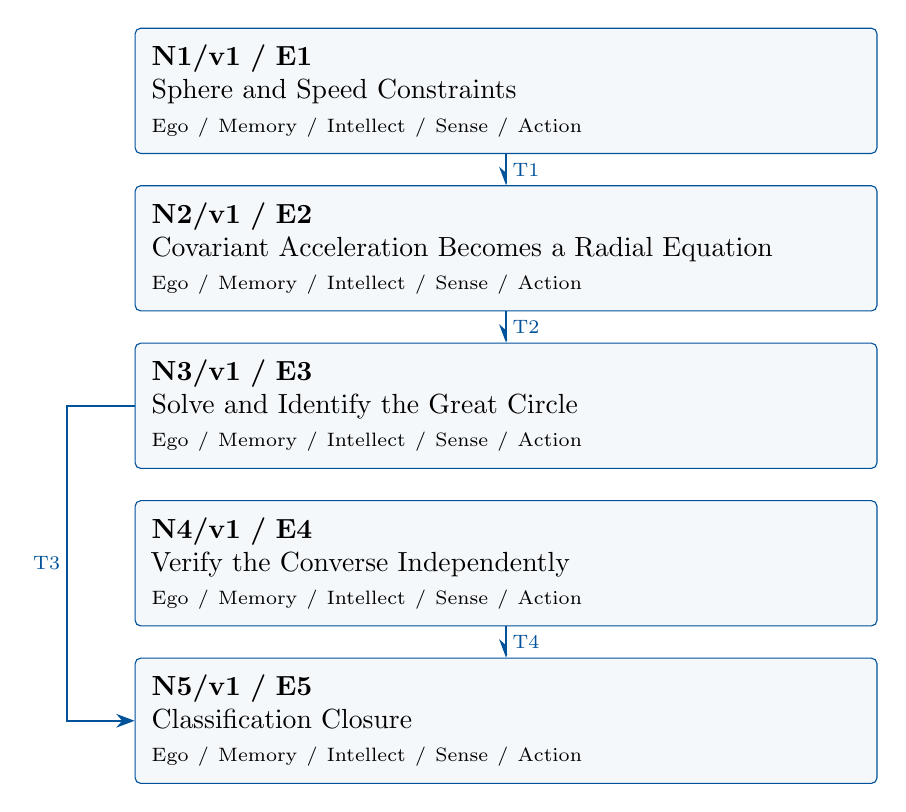
\begin{tikzpicture}[>=Stealth,x=1cm,y=1cm]

\node[mmnode,text width=9cm,minimum height=1.25cm] (N1) at (0,0.0) {\textbf{N1/v1 / E1}\\Sphere and Speed Constraints\\{\scriptsize Ego / Memory / Intellect / Sense / Action}};

\node[mmnode,text width=9cm,minimum height=1.25cm] (N2) at (0,-2.0) {\textbf{N2/v1 / E2}\\Covariant Acceleration Becomes a Radial Equation\\{\scriptsize Ego / Memory / Intellect / Sense / Action}};

\node[mmnode,text width=9cm,minimum height=1.25cm] (N3) at (0,-4.0) {\textbf{N3/v1 / E3}\\Solve and Identify the Great Circle\\{\scriptsize Ego / Memory / Intellect / Sense / Action}};

\node[mmnode,text width=9cm,minimum height=1.25cm] (N4) at (0,-6.0) {\textbf{N4/v1 / E4}\\Verify the Converse Independently\\{\scriptsize Ego / Memory / Intellect / Sense / Action}};

\node[mmnode,text width=9cm,minimum height=1.25cm] (N5) at (0,-8.0) {\textbf{N5/v1 / E5}\\Classification Closure\\{\scriptsize Ego / Memory / Intellect / Sense / Action}};

\draw[mmproof] (N1.south) -- node[mmnote,right] {T1} (N2.north);

\draw[mmproof] (N2.south) -- node[mmnote,right] {T2} (N3.north);

\draw[mmproof] (N3.west) -- (-5.58,-4) -- node[mmnote,left] {T3} (-5.58,-8) -- (N5.west);

\draw[mmproof] (N4.south) -- node[mmnote,right] {T4} (N5.north);

\end{tikzpicture}\end{center}

Each box is one mathematical agent containing all five faculties. Blue
arrows carry the versioned exports listed below. The layout gives a
reading order; only drawn arrows assert dependencies. Diagnostic repair
is separate from the proof DAG.

\clearpage\subsection{Versioned evidence-transfer ledger}

\begingroup\small\linespread{1.05}\selectfont

\Needspace{5\baselineskip}\field{T1: N1/E1/v1 to N2}{\(\langle\gamma,\gamma^{\prime}\rangle=0\) and
\(\langle\gamma,\gamma^{\prime\prime}\rangle=-1\).}

\field{Receiving activity}{N2: Covariant Acceleration Becomes a Radial Equation}

\field{Compatibility}{Use the same mathematical objects and hypotheses as the source export.
Receiving contract: N1/E1 and the tangential-projection formula for the
induced connection.}

\Needspace{5\baselineskip}\field{T2: N2/E2/v1 to N3}{\(\gamma^{\prime\prime}=-\gamma/R^2\).}

\field{Receiving activity}{N3: Solve and Identify the Great Circle}

\field{Compatibility}{Use the same mathematical objects and hypotheses as the source export.
Receiving contract: N2/E2, \(\|p\|=R\), \(\|v\|=1\), \(p\cdot v=0\), and
linear ODE uniqueness.}

\Needspace{5\baselineskip}\field{T3: N3/E3/v1 to N5}{\(\gamma(s)=p\cos(s/R)+Rv\sin(s/R)\), contained in the origin plane
spanned by \(p,v\).}

\field{Receiving activity}{N5: Classification Closure}

\field{Compatibility}{Use the same mathematical objects and hypotheses as the source export.
Receiving contract: N3/E3 and N4/E4.}

\Needspace{5\baselineskip}\field{T4: N4/E4/v1 to N5}{Every unit-speed great-circle parametrization is a geodesic.}

\field{Receiving activity}{N5: Classification Closure}

\field{Compatibility}{Use the same mathematical objects and hypotheses as the source export.
Receiving contract: N3/E3 and N4/E4.}

\endgroup

\clearpage\section{Agent roles and five-faculty activities}\begingroup\small\linespread{1.05}\selectfont\setlist{itemsep=1pt,topsep=2pt}

\subsection{N1/v1: Sphere and Speed Constraints}

\field{Object and role}{Sphere and Speed Constraints. Establish the following local result:
\(\langle\gamma,\gamma^{\prime}\rangle=0\) and
\(\langle\gamma,\gamma^{\prime\prime}\rangle=-1\).}

\field{Inputs}{A \(C^2\) unit-speed geodesic on the sphere of radius \(R>0\).}

\mmfaculty{E}{Ego}{Own E1/v1: \(\langle\gamma,\gamma^{\prime}\rangle=0\) and
\(\langle\gamma,\gamma^{\prime\prime}\rangle=-1\).}

\mmfaculty{M}{Memory}{Round metric and arc length}

\mmfaculty{I}{Intellect}{Fix point and tangent data}

\mmfaculty{S}{Sense}{Require \(R>0\) and unit speed}

\mmfaculty{A}{Action}{Carry out the numbered deductions and publish E1/v1 together with its
hypotheses and proof location.}

\smallskip\noindent\textbf{Numbered mathematical activities}

\begin{enumerate}[label=N1.\arabic*,leftmargin=3.4em]

\item Differentiate \(\langle\gamma,\gamma\rangle=R^2\) once and twice.

\item Use \(\|\gamma^{\prime}\|^2=1\).

\item Retain both tangent and acceleration constraints along the parameter
interval.

\end{enumerate}

\field{Export E1/v1}{\(\langle\gamma,\gamma^{\prime}\rangle=0\) and
\(\langle\gamma,\gamma^{\prime\prime}\rangle=-1\).}

\field{Acceptance gate}{Require \(R>0\) and unit speed Publish only after checking every
displayed deduction.}

\field{Targeted repair}{If the check fails, revise N1: Require \(R>0\) and unit speed Recheck
dependent nodes N2, N3, N5.}

\clearpage

\subsection{N2/v1: Covariant Acceleration Becomes a Radial Equation}

\field{Object and role}{Covariant Acceleration Becomes a Radial Equation. Establish the
following local result: \(\gamma^{\prime\prime}=-\gamma/R^2\).}

\field{Inputs}{N1/E1 and the tangential-projection formula for the induced connection.}

\mmfaculty{E}{Ego}{Own E2/v1: \(\gamma^{\prime\prime}=-\gamma/R^2\).}

\mmfaculty{M}{Memory}{Tangential-projection connection}

\mmfaculty{I}{Intellect}{Use normal-line characterization}

\mmfaculty{S}{Sense}{Separate ambient and intrinsic derivatives}

\mmfaculty{A}{Action}{Carry out the numbered deductions and publish E2/v1 together with its
hypotheses and proof location.}

\smallskip\noindent\textbf{Numbered mathematical activities}

\begin{enumerate}[label=N2.\arabic*,leftmargin=3.4em]

\item Zero covariant acceleration makes ambient acceleration normal.

\item The normal line is spanned by \(\gamma\).

\item Pair \(\gamma^{\prime\prime}=\lambda\gamma\) with \(\gamma\) to obtain
\(\lambda=-1/R^2\).

\end{enumerate}

\field{Export E2/v1}{\(\gamma^{\prime\prime}=-\gamma/R^2\).}

\field{Acceptance gate}{Separate ambient and intrinsic derivatives Publish only after checking
every displayed deduction.}

\field{Targeted repair}{If the check fails, revise N2: Separate ambient and intrinsic
derivatives Recheck dependent nodes N3, N5.}

\clearpage

\subsection{N3/v1: Solve and Identify the Great Circle}

\field{Object and role}{Solve and Identify the Great Circle. Establish the following local
result: \(\gamma(s)=p\cos(s/R)+Rv\sin(s/R)\), contained in the origin
plane spanned by \(p,v\).}

\field{Inputs}{N2/E2, \(\|p\|=R\), \(\|v\|=1\), \(p\cdot v=0\), and linear ODE
uniqueness.}

\mmfaculty{E}{Ego}{Own E3/v1: \(\gamma(s)=p\cos(s/R)+Rv\sin(s/R)\), contained in the origin
plane spanned by \(p,v\).}

\mmfaculty{M}{Memory}{Linear ODE solution}

\mmfaculty{I}{Intellect}{Solve oscillator}

\mmfaculty{S}{Sense}{Respect initial constraints}

\mmfaculty{A}{Action}{Carry out the numbered deductions and publish E3/v1 together with its
hypotheses and proof location.}

\smallskip\noindent\textbf{Numbered mathematical activities}

\begin{enumerate}[label=N3.\arabic*,leftmargin=3.4em]

\item Solve the constant-coefficient oscillator with the initial point and
tangent.

\item Write \(e_1=p/R\) and \(e_2=v\), an orthonormal pair.

\item Identify the intersection of their plane with the sphere.

\end{enumerate}

\field{Export E3/v1}{\(\gamma(s)=p\cos(s/R)+Rv\sin(s/R)\), contained in the origin plane
spanned by \(p,v\).}

\field{Acceptance gate}{Respect initial constraints Publish only after checking every displayed
deduction.}

\field{Targeted repair}{If the check fails, revise N3: Respect initial constraints Recheck
dependent nodes N5.}

\clearpage

\subsection{N4/v1: Verify the Converse Independently}

\field{Object and role}{Verify the Converse Independently. Establish the following local result:
Every unit-speed great-circle parametrization is a geodesic.}

\field{Inputs}{Any orthonormal pair \(e_1,e_2\) and the round sphere metric; no forward
classification is assumed.}

\mmfaculty{E}{Ego}{Own E4/v1: Every unit-speed great-circle parametrization is a geodesic.}

\mmfaculty{M}{Memory}{Great-circle parametrization}

\mmfaculty{I}{Intellect}{Compute tangential acceleration}

\mmfaculty{S}{Sense}{Require orthonormal directions}

\mmfaculty{A}{Action}{Carry out the numbered deductions and publish E4/v1 together with its
hypotheses and proof location.}

\smallskip\noindent\textbf{Numbered mathematical activities}

\begin{enumerate}[label=N4.\arabic*,leftmargin=3.4em]

\item Differentiate \(R(e_1\cos(s/R)+e_2\sin(s/R))\).

\item Check sphere membership, unit speed, and acceleration \(-\gamma/R^2\).

\item The acceleration has zero tangential projection.

\end{enumerate}

\field{Export E4/v1}{Every unit-speed great-circle parametrization is a geodesic.}

\field{Acceptance gate}{Require orthonormal directions Publish only after checking every
displayed deduction.}

\field{Targeted repair}{If the check fails, revise N4: Require orthonormal directions Recheck
dependent nodes N5.}

\clearpage

\subsection{N5/v1: Classification Closure}

\field{Object and role}{Classification Closure. Establish the following local result: Unit-speed
geodesics on the round sphere are exactly unit-speed great-circle arcs.}

\field{Inputs}{N3/E3 and N4/E4.}

\mmfaculty{E}{Ego}{Own E5/v1: Unit-speed geodesics on the round sphere are exactly
unit-speed great-circle arcs.}

\mmfaculty{M}{Memory}{Both proof branches}

\mmfaculty{I}{Intellect}{Join necessity and converse}

\mmfaculty{S}{Sense}{Avoid global minimizing overclaim}

\mmfaculty{A}{Action}{Carry out the numbered deductions and publish E5/v1 together with its
hypotheses and proof location.}

\smallskip\noindent\textbf{Numbered mathematical activities}

\begin{enumerate}[label=N5.\arabic*,leftmargin=3.4em]

\item Combine necessity and sufficiency.

\item Use ODE uniqueness for the initial-data classification.

\item Separate this geodesic statement from the stronger and generally false
claim that every whole arc is globally shortest.

\end{enumerate}

\field{Export E5/v1}{Unit-speed geodesics on the round sphere are exactly unit-speed
great-circle arcs.}

\field{Acceptance gate}{Avoid global minimizing overclaim Publish only after checking every
displayed deduction.}

\field{Targeted repair}{If the check fails, revise N5: Avoid global minimizing overclaim
Withhold this terminal result until its gate passes.}

\endgroup\clearpage\section{Continuous mathematical proof}\label{sec:proof}

\subsection{N1 --- Sphere and Speed
Constraints}\label{n1-sphere-and-speed-constraints}

Let \(\gamma (s)\) be a unit-speed geodesic. The sphere and speed
conditions are

\[\langle\gamma,\gamma\rangle=R^2,\qquad\langle\gamma',\gamma'\rangle=1.\]

Differentiating the first once gives \(\langle\gamma,\gamma'\rangle=0\),
so velocity is tangent. Differentiating again gives

\[\langle\gamma,\gamma''\rangle=-\langle\gamma',\gamma'\rangle=-1.\]

These identities are valid along the whole curve.

\subsection{N2 --- Covariant Acceleration Becomes a Radial
Equation}\label{n2-covariant-acceleration-becomes-a-radial-equation}

The geodesic condition says the tangential projection of gamma'\,' is
zero. The normal line at gamma is spanned by gamma itself. Hence
\(\gamma''=\lambda(s)\gamma\). Taking inner products with gamma and
using N1 gives \(\lambda(s)R^2=-1\), so

\[\gamma''=-\frac1{R^2}\gamma.\]

This nonzero inward acceleration keeps a geodesic on the curved sphere
while its intrinsic acceleration vanishes.

\subsection{N3 --- Solve and Identify the Great
Circle}\label{n3-solve-and-identify-the-great-circle}

At \(s=0\) choose initial point p and unit tangent v, so
\(\Vert p\Vert =R\), \(\Vert v\Vert =1\), and \(p\cdot v=0\). The unique
solution of N2's ODE with these data is

\[\gamma(s)=p\cos(s/R)+Rv\sin(s/R).\]

Its image stays in the fixed plane span (p,v), which passes through the
origin. Writing \(e_{1}=p/R\) and \(e_{2}=v\) gives an orthonormal pair
and

\[\gamma(s)=R\big(e_1\cos(s/R)+e_2\sin(s/R)\big).\]

It therefore traces a great-circle arc. Any other initial parameter
value can be shifted to zero, so this covers every unit-speed geodesic
locally and throughout its parameter interval by uniqueness.

\subsection{N4 --- Verify the Converse
Independently}\label{n4-verify-the-converse-independently}

Given any orthonormal \(e_{1},e_{2}\), the last formula satisfies
\(\Vert \gamma \Vert =R\), \textbar\textbar gamma'\(\Vert =1\), and
gamma'\,'\(=-\gamma /R^{2}\). Its acceleration is normal to the sphere,
so its tangential projection is zero. The curve is a geodesic. This
check does not assume the forward classification.

\subsection{N5 --- Classification
Closure}\label{n5-classification-closure}

N3 proves necessity and N4 proves sufficiency. Initial data determine a
unique parameterized geodesic, while reversing the tangent reverses
direction along the same great circle. The theorem follows. \(\square\)

\hfill$\square$

\section{Worked orchestration}

On the unit sphere, \(p=(1,0,0)\), \(v=(0,1,0)\) gives

\[\gamma(s)=(\cos s,\sin s,0),\]

the equator. Ambient acceleration is \(-\gamma\), entirely normal, while
speed is one.

Now consider a latitude with \(0<|c|<1\). Let \(\rho =sqrt(1-c^{2})\)
and

\[\eta(s)=(\rho\cos(s/\rho),\rho\sin(s/\rho),c).\]

This is unit speed. Its ambient acceleration is

\[\eta''=(-\cos(s/\rho)/\rho,-\sin(s/\rho)/\rho,0).\]

Since eta \(\cdot eta\)'\,`\(=-1\), its tangential component on the unit
sphere is eta'\,'+eta. Its third coordinate is c, so this component is
nonzero. The latitude is not a geodesic. When \(c=0\), \(\rho =1\) and
the tangential acceleration vanishes, recovering the equator.

\subsection{Boundary and hypothesis audit}

Unit speed matters: for constant speed \(c_{0}\) the equation becomes
gamma'\,'\(=-c_{0}^{2}\) \(\gamma /R^{2}\). Arbitrary
reparameterizations may not satisfy the affine geodesic equation even
when their images remain great circles. Constant geodesics are excluded
by the nonconstant unit-speed contract.

A geodesic arc need not minimize length globally. On a unit great
circle, an arc of length \(3\pi /2\) has the same endpoints as the
opposite arc of length \(\pi /2\). Antipodal endpoints admit multiple
semicircular geodesics. Neither fact contradicts the classification.

Export the normal-acceleration bridge, the initial-value formula, and
the great-circle equivalence. These supply concrete local geodesic
intuition for later completeness and curvature problems.

\section{Illustrative failure and repair}

The following is an authored diagnostic scenario. Changed assumptions
define a new contract; they do not retroactively prove the original
statement.

\subsection{Failure and correction}
A branch identifies all geodesics with straight lines because it
replaces covariant acceleration by ordinary acceleration.

\begin{itemize}
\item
  \textbf{Node:} N2
\item
  \textbf{State:} STALLED
\item
  \textbf{Failing faculty:} Sense
\item
  \textbf{Failed definition:} geodesic means zero tangential
  acceleration
\item
  \textbf{Observed:} ambient acceleration incorrectly set to zero
\item
  \textbf{Repair target:} connection interpretation
\item
  \textbf{Blocked export:} straight-line classification
\end{itemize}

Memory retrieves the induced connection. Sense distinguishes the two
derivatives. Intellect uses normal acceleration instead of zero ambient
acceleration. Action derives gamma'\,'\(=-\gamma /R^{2}\) and verifies
the equator. Ego retains the classification target and replaces the
invalid bridge.

\subsection{Hypothesis boundary}
Unit speed matters: for constant speed \(c_{0}\) the equation becomes
gamma'\,'\(=-c_{0}^{2}\) \(\gamma /R^{2}\). Arbitrary
reparameterizations may not satisfy the affine geodesic equation even
when their images remain great circles. Constant geodesics are excluded
by the nonconstant unit-speed contract.

A geodesic arc need not minimize length globally. On a unit great
circle, an arc of length \(3\pi /2\) has the same endpoints as the
opposite arc of length \(\pi /2\). Antipodal endpoints admit multiple
semicircular geodesics. Neither fact contradicts the classification.

Export the normal-acceleration bridge, the initial-value formula, and
the great-circle equivalence. These supply concrete local geodesic
intuition for later completeness and curvature problems.

\subsection{Version and recheck}
Treat any changed assumption as a new contract. Recheck the revised
export and all of its descendants. A backward diagnostic never
establishes an earlier theorem. This is an authored teaching trace, not
an execution log.

\par\medskip\begingroup\small\linespread{1.0}\selectfont\noindent\textbf{Provenance.} This authored proof is complete relative to its declared imports. Reuse
each export with its assumptions, proof, and version. The original
Markdown remains available for comparison.
\par\endgroup

\par\smallskip\begingroup\small\linespread{1.0}\selectfont\noindent\textbf{Further reading.} \href{https://people.math.harvard.edu/~landesman/assets/math-230a-harvard-differential-geometry-notes.pdf}{Harvard
differential geometry notes: induced connections and geodesics}.\par\endgroup

\end{document}
